\chapter{Vjerojatnost}

\index{vjerojatnost}

\key{Vjerojatnost} je realan broj između $0$ i $1$
koji pokazuje koliko je neki događaj vjerojatan.
Ako se događaj sigurno dogodi,
njegova vjerojatnost je 1,
a ako je događaj nemoguć,
njegova vjerojatnost je 0.
Vjerojatnost događaja označavamo $P(\cdots)$
gdje tri točkice opisuju događaj.

Na primjer, pri bacanju kocke,
ishod je cijeli broj između $1$ i $6$,
a vjerojatnost svakog ishoda je $1/6$.
Na primjer, možemo izračunati sljedeće vjerojatnosti:

\begin{itemize}[noitemsep]
\item $P(\textrm{''ishod je 4''})=1/6$
\item $P(\textrm{''ishod nije 6''})=5/6$
\item $P(\textrm{''ishod je paran''})=1/2$
\end{itemize}

\section{Izračunavanje}

Da bismo izračunali vjerojatnost događaja,
možemo koristiti kombinatoriku
ili simulirati proces koji generira događaj.
Kao primjer, izračunajmo vjerojatnost
izvlačenja triju karata iste vrijednosti
iz promiješanog špila karata
(na primjer, $\spadesuit 8$, $\clubsuit 8$ i $\diamondsuit 8$).

\subsubsection*{Metoda 1}

Vjerojatnost možemo izračunati pomoću formule

\[\frac{\textrm{broj željenih ishoda}}{\textrm{ukupan broj ishoda}}.\]

U ovom zadatku, željeni ishodi su oni
u kojima je vrijednost svake karte jednaka.
Postoji $13 {4 \choose 3}$ takvih ishoda,
jer postoji $13$ mogućnosti za
vrijednost karata i ${4 \choose 3}$ načina da
odaberemo $3$ boje od $4$ moguće boje.

Ukupno postoji ${52 \choose 3}$ ishoda,
jer biramo 3 karte od 52 karte.
Dakle, vjerojatnost događaja je

\[\frac{13 {4 \choose 3}}{{52 \choose 3}} = \frac{1}{425}.\]

\subsubsection*{Metoda 2}

Drugi način izračunavanja vjerojatnosti je
simuliranje procesa koji generira događaj.
U ovom primjeru izvlačimo tri karte, pa se proces
sastoji od tri koraka.
Zahtijevamo da svaki korak procesa bude uspješan.

Izvlačenje prve karte sigurno uspijeva,
jer nema nikakvih ograničenja.
Drugi korak uspijeva s vjerojatnošću $3/51$,
jer je preostala 51 karta i 3 od njih
imaju istu vrijednost kao prva karta.
Na sličan način, treći korak uspijeva s vjerojatnošću $2/50$.

Vjerojatnost da cijeli proces uspije je

\[1 \cdot \frac{3}{51} \cdot \frac{2}{50} = \frac{1}{425}.\]

\section{Događaji}

Događaj u teoriji vjerojatnosti može se prikazati kao skup
\[A \subset X,\]
gdje $X$ sadrži sve moguće ishode,
a $A$ je podskup ishoda.
Na primjer, pri bacanju kocke, ishodi su
\[X = \{1,2,3,4,5,6\}.\]
Sada, na primjer, događaj ''ishod je paran''
odgovara skupu
\[A = \{2,4,6\}.\]

Svakom ishodu $x$ pridružena je vjerojatnost $p(x)$.
Tada se vjerojatnost $P(A)$ događaja
$A$ može izračunati kao suma
vjerojatnosti ishoda pomoću formule
\[P(A) = \sum_{x \in A} p(x).\]
Na primjer, pri bacanju kocke,
$p(x)=1/6$ za svaki ishod $x$,
pa je vjerojatnost događaja
''ishod je paran''
\[p(2)+p(4)+p(6)=1/2.\]

Ukupna vjerojatnost ishoda u $X$ mora
biti 1, tj. $P(X)=1$.

Budući da su događaji u teoriji vjerojatnosti skupovi,
možemo njima manipulirati pomoću standardnih skupovnih operacija:

\begin{itemize}
\item \key{Komplement} $\bar A$ znači
''$A$ se ne dogodi''.
Na primjer, pri bacanju kocke,
komplement od $A=\{2,4,6\}$ je
$\bar A = \{1,3,5\}$.
\item \key{Unija} $A \cup B$ znači
''$A$ ili $B$ se dogodi''.
Na primjer, unija od
$A=\{2,5\}$
i $B=\{4,5,6\}$ je
$A \cup B = \{2,4,5,6\}$.
\item \key{Presjek} $A \cap B$ znači
''$A$ i $B$ se dogode''.
Na primjer, presjek od
$A=\{2,5\}$ i $B=\{4,5,6\}$ je
$A \cap B = \{5\}$.
\end{itemize}

\subsubsection{Komplement}

Vjerojatnost komplementa
$\bar A$ izračunava se pomoću formule
\[P(\bar A)=1-P(A).\]

Ponekad možemo lako riješiti zadatak
pomoću komplemenata tako da riješimo suprotan zadatak.
Na primjer, vjerojatnost da dobijemo
barem jednu šesticu pri bacanju kocke deset puta je
\[1-(5/6)^{10}.\]

Ovdje je $5/6$ vjerojatnost da ishod
jednog bacanja nije šestica, a
$(5/6)^{10}$ je vjerojatnost da nijedno od
deset bacanja nije šestica.
Komplement toga je odgovor na zadatak.

\subsubsection{Unija}

Vjerojatnost unije $A \cup B$
izračunava se pomoću formule
\[P(A \cup B)=P(A)+P(B)-P(A \cap B).\]
Na primjer, pri bacanju kocke,
unija događaja
\[A=\textrm{''ishod je paran''}\]
i
\[B=\textrm{''ishod je manji od 4''}\]
je
\[A \cup B=\textrm{''ishod je paran ili manji od 4''},\]
a njezina vjerojatnost je
\[P(A \cup B) = P(A)+P(B)-P(A \cap B)=1/2+1/2-1/6=5/6.\]

Ako su događaji $A$ i $B$ \key{disjunktni}, tj.
$A \cap B$ je prazan,
vjerojatnost događaja $A \cup B$ je jednostavno

\[P(A \cup B)=P(A)+P(B).\]

\subsubsection{Uvjetna vjerojatnost}

\index{uvjetna vjerojatnost}

\key{Uvjetna vjerojatnost}
\[P(A | B) = \frac{P(A \cap B)}{P(B)}\]
je vjerojatnost događaja $A$
uz pretpostavku da se $B$ dogodi.
Dakle, pri izračunavanju
vjerojatnosti događaja $A$, razmatramo samo ishode
koji također pripadaju $B$.

Koristeći prethodne skupove,
\[P(A | B)= 1/3,\]
jer su ishodi od $B$
$\{1,2,3\}$, a jedan od njih je paran.
To je vjerojatnost parnog ishoda
ako znamo da je ishod između $1 \ldots 3$.

\subsubsection{Presjek}

\index{nezavisnost}

Koristeći uvjetnu vjerojatnost,
vjerojatnost presjeka
$A \cap B$ može se izračunati pomoću formule
\[P(A \cap B)=P(A)P(B|A).\]
Događaji $A$ i $B$ su \key{nezavisni} ako
\[P(A|B)=P(A) \hspace{10px}\textrm{i}\hspace{10px} P(B|A)=P(B),\]
što znači da činjenica da se $B$ dogodi ne
mijenja vjerojatnost događaja $A$, i obrnuto.
U tom slučaju, vjerojatnost presjeka je
\[P(A \cap B)=P(A)P(B).\]
Na primjer, pri izvlačenju karte iz špila, događaji
\[A = \textrm{''boja je tref''}\]
i
\[B = \textrm{''vrijednost je četiri''}\]
su nezavisni. Stoga se događaj
\[A \cap B = \textrm{''karta je tref četvorka''}\]
dogodi s vjerojatnošću
\[P(A \cap B)=P(A)P(B)=1/4 \cdot 1/13 = 1/52.\]

\section{Slučajne varijable}

\index{slučajna varijabla}

\key{Slučajna varijabla} je vrijednost koju generira
slučajan proces.
Na primjer, pri bacanju dviju kocaka,
moguća slučajna varijabla je
\[X=\textrm{''suma ishoda''}.\]
Na primjer, ako su ishodi $[4,6]$
(što znači da smo prvo bacili četvorku, a zatim šesticu),
tada je vrijednost od $X$ jednaka 10.

S $P(X=x)$ označavamo vjerojatnost da
je vrijednost slučajne varijable $X$ jednaka $x$.
Na primjer, pri bacanju dviju kocaka,
$P(X=10)=3/36$,
jer je ukupan broj ishoda 36,
a postoje tri moguća načina da dobijemo
sumu 10: $[4,6]$, $[5,5]$ i $[6,4]$.

\subsubsection{Očekivana vrijednost}

\index{očekivana vrijednost}

\key{Očekivana vrijednost} $E[X]$ pokazuje
prosječnu vrijednost slučajne varijable $X$.
Očekivana vrijednost može se izračunati kao suma
\[\sum_x P(X=x)x,\]
gdje $x$ prolazi kroz sve moguće vrijednosti od $X$.

Na primjer, pri bacanju kocke,
očekivani ishod je
\[1/6 \cdot 1 + 1/6 \cdot 2 + 1/6 \cdot 3 + 1/6 \cdot 4 + 1/6 \cdot 5 + 1/6 \cdot 6 = 7/2.\]

Korisno svojstvo očekivanih vrijednosti je \key{linearnost}.
Ona znači da je suma
$E[X_1+X_2+\cdots+X_n]$
uvijek jednaka sumi
$E[X_1]+E[X_2]+\cdots+E[X_n]$.
Ova formula vrijedi čak i ako slučajne varijable
ovise jedna o drugoj.

Na primjer, pri bacanju dviju kocaka,
očekivana suma je
\[E[X_1+X_2]=E[X_1]+E[X_2]=7/2+7/2=7.\]

Razmotrimo sada zadatak u kojem se
$n$ kuglica nasumično stavlja u $n$ kutija,
a naš je zadatak izračunati očekivani
broj praznih kutija.
Svaka kuglica ima jednaku vjerojatnost da
bude stavljena u bilo koju od kutija.
Na primjer, ako je $n=2$, mogućnosti
su sljedeće:
\begin{center}
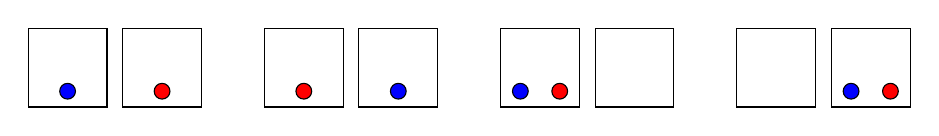
\begin{tikzpicture}
\draw (0,0) rectangle (1,1);
\draw (1.2,0) rectangle (2.2,1);
\draw (3,0) rectangle (4,1);
\draw (4.2,0) rectangle (5.2,1);
\draw (6,0) rectangle (7,1);
\draw (7.2,0) rectangle (8.2,1);
\draw (9,0) rectangle (10,1);
\draw (10.2,0) rectangle (11.2,1);

\draw[fill=blue] (0.5,0.2) circle (0.1);
\draw[fill=red] (1.7,0.2) circle (0.1);
\draw[fill=red] (3.5,0.2) circle (0.1);
\draw[fill=blue] (4.7,0.2) circle (0.1);
\draw[fill=blue] (6.25,0.2) circle (0.1);
\draw[fill=red] (6.75,0.2) circle (0.1);
\draw[fill=blue] (10.45,0.2) circle (0.1);
\draw[fill=red] (10.95,0.2) circle (0.1);
\end{tikzpicture}
\end{center}
U ovom slučaju, očekivani broj
praznih kutija je
\[\frac{0+0+1+1}{4} = \frac{1}{2}.\]
U općem slučaju, vjerojatnost da je
jedna kutija prazna je
\[\Big(\frac{n-1}{n}\Big)^n,\]
jer u nju ne smije biti stavljena nijedna kuglica.
Stoga je, koristeći linearnost, očekivani broj
praznih kutija
\[n \cdot \Big(\frac{n-1}{n}\Big)^n.\]

\subsubsection{Distribucije}

\index{distribucija}

\key{Distribucija} slučajne varijable $X$
pokazuje vjerojatnost svake vrijednosti koju
$X$ može imati.
Distribucija se sastoji od vrijednosti $P(X=x)$.
Na primjer, pri bacanju dviju kocaka,
distribucija njihove sume je:
\begin{center}
\small {
\begin{tabular}{r|rrrrrrrrrrrrr}
$x$ & 2 & 3 & 4 & 5 & 6 & 7 & 8 & 9 & 10 & 11 & 12 \\
$P(X=x)$ & $1/36$ & $2/36$ & $3/36$ & $4/36$ & $5/36$ & $6/36$ & $5/36$ & $4/36$ & $3/36$ & $2/36$ & $1/36$ \\
\end{tabular}
}
\end{center}

\index{uniformna distribucija}
U \key{uniformnoj distribuciji},
slučajna varijabla $X$ ima $n$ mogućih
vrijednosti $a,a+1,\ldots,b$, a vjerojatnost svake vrijednosti je $1/n$.
Na primjer, pri bacanju kocke,
$a=1$, $b=6$ i $P(X=x)=1/6$ za svaku vrijednost $x$.

Očekivana vrijednost od $X$ u uniformnoj distribuciji je
\[E[X] = \frac{a+b}{2}.\]

\index{binomna distribucija}
U \key{binomnoj distribuciji}, izvodi se $n$ pokušaja,
a vjerojatnost da pojedini pokušaj uspije
je $p$.
Slučajna varijabla $X$ broji
uspješne pokušaje,
a vjerojatnost vrijednosti $x$ je
\[P(X=x)=p^x (1-p)^{n-x} {n \choose x},\]
gdje $p^x$ i $(1-p)^{n-x}$ odgovaraju
uspješnim i neuspješnim pokušajima,
a ${n \choose x}$ je broj načina na koje
možemo odabrati redoslijed pokušaja.

Na primjer, pri bacanju kocke deset puta,
vjerojatnost da bacimo šesticu točno
tri puta je $(1/6)^3 (5/6)^7 {10 \choose 3}$.

Očekivana vrijednost od $X$ u binomnoj distribuciji je
\[E[X] = pn.\]

\index{geometrijska distribucija}
U \key{geometrijskoj distribuciji},
vjerojatnost da pokušaj uspije je $p$,
a nastavljamo dok se ne dogodi prvi uspjeh.
Slučajna varijabla $X$ broji
potrebne pokušaje, a vjerojatnost
vrijednosti $x$ je
\[P(X=x)=(1-p)^{x-1} p,\]
gdje $(1-p)^{x-1}$ odgovara neuspješnim pokušajima,
a $p$ odgovara prvom uspješnom pokušaju.

Na primjer, ako bacamo kocku dok ne bacimo šesticu,
vjerojatnost da je broj bacanja
točno 4 iznosi $(5/6)^3 1/6$.

Očekivana vrijednost od $X$ u geometrijskoj distribuciji je
\[E[X]=\frac{1}{p}.\]

\section{Markovljevi lanci}

\index{Markovljev lanac}

\key{Markovljev lanac}
% \footnote{A. A. Markov (1856--1922)
% was a Russian mathematician.}
je slučajan proces
koji se sastoji od stanja i prijelaza između njih.
Za svako stanje znamo vjerojatnosti
prelaska u druga stanja.
Markovljev lanac može se prikazati kao graf
čiji su čvorovi stanja, a bridovi prijelazi.

Kao primjer, razmotrimo zadatak
u kojem se nalazimo na katu 1 zgrade od $n$ katova.
U svakom koraku nasumično idemo ili jedan kat
gore ili jedan kat dolje, osim što uvijek
idemo jedan kat gore s kata 1 i jedan kat dolje
s kata $n$.
Kolika je vjerojatnost da smo na katu $m$
nakon $k$ koraka?

U ovom zadatku, svaki kat zgrade
odgovara stanju u Markovljevom lancu.
Na primjer, ako je $n=5$, graf je sljedeći:

\begin{center}
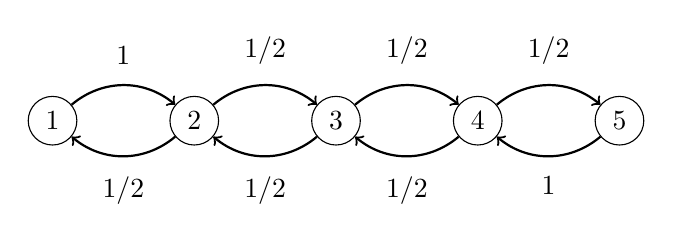
\begin{tikzpicture}[scale=0.9]
\node[draw, circle] (1) at (0,0) {$1$};
\node[draw, circle] (2) at (2,0) {$2$};
\node[draw, circle] (3) at (4,0) {$3$};
\node[draw, circle] (4) at (6,0) {$4$};
\node[draw, circle] (5) at (8,0) {$5$};

\path[draw,thick,->] (1) edge [bend left=40] node[font=\small,label=$1$] {} (2);
\path[draw,thick,->] (2) edge [bend left=40] node[font=\small,label=$1/2$] {} (3);
\path[draw,thick,->] (3) edge [bend left=40] node[font=\small,label=$1/2$] {} (4);
\path[draw,thick,->] (4) edge [bend left=40] node[font=\small,label=$1/2$] {} (5);

\path[draw,thick,->] (5) edge [bend left=40] node[font=\small,label=below:$1$] {} (4);
\path[draw,thick,->] (4) edge [bend left=40] node[font=\small,label=below:$1/2$] {} (3);
\path[draw,thick,->] (3) edge [bend left=40] node[font=\small,label=below:$1/2$] {} (2);
\path[draw,thick,->] (2) edge [bend left=40] node[font=\small,label=below:$1/2$] {} (1);

%\path[draw,thick,->] (1) edge [bend left=40] node[font=\small,label=below:$1$] {} (2);
\end{tikzpicture}
\end{center}

Distribucija vjerojatnosti
Markovljevog lanca je vektor
$[p_1,p_2,\ldots,p_n]$, gdje je $p_k$
vjerojatnost da je trenutno stanje $k$.
Formula $p_1+p_2+\cdots+p_n=1$ uvijek vrijedi.

U gornjem scenariju, početna distribucija je
$[1,0,0,0,0]$, jer uvijek počinjemo na katu 1.
Sljedeća distribucija je $[0,1,0,0,0]$,
jer se s kata 1 možemo pomaknuti samo na kat 2.
Nakon toga se možemo pomaknuti ili jedan kat gore
ili jedan kat dolje, pa je sljedeća distribucija
$[1/2,0,1/2,0,0]$, i tako dalje.

Efikasan način simuliranja šetnje u
Markovljevom lancu je korištenje dinamičkog programiranja.
Ideja je održavati distribuciju vjerojatnosti
i u svakom koraku proći kroz sve mogućnosti
kako se možemo pomaknuti.
Koristeći ovu metodu, možemo simulirati
šetnju od $m$ koraka u $O(n^2 m)$ vremenu.

Prijelazi Markovljevog lanca mogu se također
prikazati kao matrica koja ažurira
distribuciju vjerojatnosti.
U gornjem scenariju, matrica je

\[ 
 \begin{bmatrix}
  0 & 1/2 & 0 & 0 & 0 \\
  1 & 0 & 1/2 & 0 & 0 \\
  0 & 1/2 & 0 & 1/2 & 0 \\
  0 & 0 & 1/2 & 0 & 1 \\
  0 & 0 & 0 & 1/2 & 0 \\
 \end{bmatrix}.
\]

Kada distribuciju vjerojatnosti pomnožimo ovom matricom,
dobivamo novu distribuciju nakon jednog koraka.
Na primjer, možemo prijeći iz distribucije
$[1,0,0,0,0]$ u distribuciju
$[0,1,0,0,0]$ na sljedeći način:

\[ 
 \begin{bmatrix}
  0 & 1/2 & 0 & 0 & 0 \\
  1 & 0 & 1/2 & 0 & 0 \\
  0 & 1/2 & 0 & 1/2 & 0 \\
  0 & 0 & 1/2 & 0 & 1 \\
  0 & 0 & 0 & 1/2 & 0 \\
 \end{bmatrix}
 \begin{bmatrix}
  1 \\
  0 \\
  0 \\
  0 \\
  0 \\
 \end{bmatrix}
=
 \begin{bmatrix}
  0 \\
  1 \\
  0 \\
  0 \\
  0 \\
 \end{bmatrix}.
\]

Efikasnim izračunavanjem potencija matrice
možemo izračunati distribuciju nakon $m$ koraka
u $O(n^3 \log m)$ vremenu.

\section{Randomizirani algoritmi}

\index{randomizirani algoritam}

Ponekad možemo koristiti slučajnost za rješavanje zadatka,
čak i ako zadatak nije povezan s vjerojatnostima.
\key{Randomizirani algoritam} je algoritam koji
se temelji na slučajnosti.

\index{Monte Carlo algoritam}

\key{Monte Carlo algoritam} je randomizirani algoritam
koji ponekad može dati pogrešan odgovor.
Da bi takav algoritam bio koristan,
vjerojatnost pogrešnog odgovora treba biti mala.

\index{Las Vegas algoritam}

\key{Las Vegas algoritam} je randomizirani algoritam
koji uvijek daje točan odgovor,
ali njegovo vrijeme izvođenja slučajno varira.
Cilj je osmisliti algoritam koji je
efikasan s velikom vjerojatnošću.

Zatim ćemo proći kroz tri primjera zadataka koji
se mogu riješiti korištenjem slučajnosti.

\subsubsection{Uređajne statistike}

\index{uređajna statistika}

$k$-ta \key{uređajna statistika} niza
je element na poziciji $k$ nakon sortiranja
niza u rastućem poretku.
Lako je izračunati bilo koju uređajnu statistiku
u $O(n \log n)$ vremenu tako da prvo sortiramo niz,
ali je li zaista potrebno sortirati cijeli niz
samo da bismo pronašli jedan element?

Pokazuje se da uređajne statistike možemo pronaći
pomoću randomiziranog algoritma bez sortiranja niza.
Algoritam, nazvan \key{quickselect}\footnote{Godine 1961.
C. A. R. Hoare objavio je dva algoritma koja
su u prosjeku efikasna: \index{quicksort} \index{quickselect}
\key{quicksort} \cite{hoa61a} za sortiranje nizova i
\key{quickselect} \cite{hoa61b} za pronalaženje uređajnih statistika.}, je Las Vegas algoritam:
njegovo vrijeme izvođenja obično je $O(n)$,
ali $O(n^2)$ u najgorem slučaju.

Algoritam odabire slučajan element $x$
niza i pomiče elemente manje od $x$
u lijevi dio niza,
a sve ostale elemente u desni dio niza.
To zahtijeva $O(n)$ vremena kada ima $n$ elemenata.
Pretpostavimo da lijevi dio sadrži $a$ elemenata,
a desni dio sadrži $b$ elemenata.
Ako je $a=k$, element $x$ je $k$-ta uređajna statistika.
Inače, ako je $a>k$, rekurzivno pronalazimo $k$-tu uređajnu
statistiku za lijevi dio,
a ako je $a<k$, rekurzivno pronalazimo $r$-tu uređajnu
statistiku za desni dio gdje je $r=k-a$.
Pretraživanje se nastavlja na sličan način dok element
ne bude pronađen.

Kada se svaki element $x$ odabire slučajno,
veličina niza se otprilike prepolovi u svakom koraku,
pa je vremenska složenost
pronalaženja $k$-te uređajne statistike otprilike
\[n+n/2+n/4+n/8+\cdots < 2n = O(n).\]

Najgori slučaj algoritma i dalje zahtijeva $O(n^2)$ vremena,
jer je moguće da se $x$ uvijek odabere
tako da bude jedan od najmanjih ili najvećih
elemenata niza, pa je potrebno $O(n)$ koraka.
Međutim, vjerojatnost za to je toliko mala
da se to u praksi nikada ne dogodi.

\subsubsection{Provjera množenja matrica}

\index{množenje matrica}

Naš sljedeći zadatak je \emph{provjeriti}
vrijedi li $AB=C$ kada su $A$, $B$ i $C$
matrice veličine $n \times n$.
Naravno, zadatak možemo riješiti
tako da ponovno izračunamo proizvod $AB$
(u $O(n^3)$ vremenu koristeći osnovni algoritam),
ali mogli bismo se nadati da bi provjera
odgovora bila lakša od izračunavanja ispočetka.

Pokazuje se da zadatak možemo riješiti
pomoću Monte Carlo algoritma\footnote{R. M. Freivalds objavio je
ovaj algoritam 1977. godine \cite{fre77}, a ponekad se
naziva \index{Freivaldsov algoritam} \key{Freivaldsov algoritam}.} čija
je vremenska složenost samo $O(n^2)$.
Ideja je jednostavna: odaberemo slučajan vektor
$X$ od $n$ elemenata i izračunamo matrice
$ABX$ i $CX$. Ako je $ABX=CX$, javljamo da je $AB=C$,
a inače javljamo da je $AB \neq C$.

Vremenska složenost algoritma je
$O(n^2)$, jer matrice
$ABX$ i $CX$ možemo izračunati u $O(n^2)$ vremenu.
Matricu $ABX$ možemo efikasno izračunati
koristeći prikaz $A(BX)$, pa su potrebna samo dva
množenja matrica veličine $n \times n$ i $n \times 1$.

Nedostatak algoritma je
što postoji mala šansa da algoritam
pogriješi kada javi da je $AB=C$.
Na primjer, 
\[
 \begin{bmatrix}
  6 & 8 \\
  1 & 3 \\
 \end{bmatrix}
\neq
 \begin{bmatrix}
  8 & 7 \\
  3 & 2 \\
 \end{bmatrix},
\]
ali
\[
 \begin{bmatrix}
  6 & 8 \\
  1 & 3 \\
 \end{bmatrix}
 \begin{bmatrix}
  3 \\
  6 \\
 \end{bmatrix}
=
 \begin{bmatrix}
  8 & 7 \\
  3 & 2 \\
 \end{bmatrix}
 \begin{bmatrix}
  3 \\
  6 \\
 \end{bmatrix}.
\]
Međutim, u praksi je vjerojatnost da
algoritam pogriješi mala,
a vjerojatnost možemo smanjiti
provjerom rezultata pomoću više slučajnih vektora $X$
prije nego što javimo da je $AB=C$.

\subsubsection{Bojenje grafa}

\index{bojenje}

Zadan je graf koji sadrži $n$ čvorova i $m$ bridova,
a naš je zadatak pronaći način bojenja čvorova
grafa dvjema bojama tako da
za barem $m/2$ bridova krajevi
imaju različite boje.
Na primjer, u grafu
\begin{center}
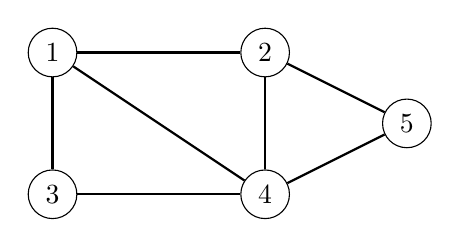
\begin{tikzpicture}[scale=0.9]
\node[draw, circle] (1) at (1,3) {$1$};
\node[draw, circle] (2) at (4,3) {$2$};
\node[draw, circle] (3) at (1,1) {$3$};
\node[draw, circle] (4) at (4,1) {$4$};
\node[draw, circle] (5) at (6,2) {$5$};

\path[draw,thick,-] (1) -- (2);
\path[draw,thick,-] (1) -- (3);
\path[draw,thick,-] (1) -- (4);
\path[draw,thick,-] (3) -- (4);
\path[draw,thick,-] (2) -- (4);
\path[draw,thick,-] (2) -- (5);
\path[draw,thick,-] (4) -- (5);
\end{tikzpicture}
\end{center}
valjano bojenje je sljedeće:
\begin{center}
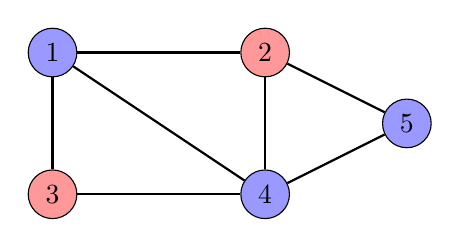
\begin{tikzpicture}[scale=0.9]
\node[draw, circle, fill=blue!40] (1) at (1,3) {$1$};
\node[draw, circle, fill=red!40] (2) at (4,3) {$2$};
\node[draw, circle, fill=red!40] (3) at (1,1) {$3$};
\node[draw, circle, fill=blue!40] (4) at (4,1) {$4$};
\node[draw, circle, fill=blue!40] (5) at (6,2) {$5$};

\path[draw,thick,-] (1) -- (2);
\path[draw,thick,-] (1) -- (3);
\path[draw,thick,-] (1) -- (4);
\path[draw,thick,-] (3) -- (4);
\path[draw,thick,-] (2) -- (4);
\path[draw,thick,-] (2) -- (5);
\path[draw,thick,-] (4) -- (5);
\end{tikzpicture}
\end{center}
Gornji graf sadrži 7 bridova, a za 5 od njih
krajevi imaju različite boje,
pa je bojenje valjano.

Zadatak se može riješiti pomoću Las Vegas algoritma
koji generira slučajna bojenja dok ne bude pronađeno
valjano bojenje.
U slučajnom bojenju, boja svakog čvora se
nezavisno odabire tako da je vjerojatnost
obiju boja $1/2$.

U slučajnom bojenju, vjerojatnost da krajevi
jednog brida imaju različite boje je $1/2$.
Stoga je očekivani broj bridova čiji krajevi
imaju različite boje $m/2$.
Budući da se očekuje da je slučajno bojenje valjano,
u praksi ćemo brzo pronaći valjano bojenje.
